\chapter{平衡}\label{ch:g2:balance-equilibrium}

跷跷板两端各坐一个孩子，它便保持水平。一座积木塔
立在那里；只要再多放一块，它就会倒塌。杂技演员走过一根
比她的鞋子还细的绳索。这三者玩的是同一个深刻的游戏：
平衡游戏——力相互抵消，什么也不动。

\section{静止即平衡}

\begin{definition}[平衡]\label{def:g2:balance-equilibrium:equilibrium}
称一个物体处于\emph{平衡}\index{平衡}状态——也说它
它是\emph{平衡的}\index{平衡的}，即作用在它身上的推力与拉力
相互抵消，它便保持原样。拔河绳上的红布条
停在两队之间纹丝不动：这就是平衡。这并不是
没有力的世界，而是力量正打成
一个完美的平手。
\end{definition}

\begin{example}[桌上的书]\label{ex:g2:balance-equilibrium:book}
一本书静静地放在桌上。无聊吗？再用上一章的眼光仔细看看。
地球把书往下拉，那它为什么
不掉下去呢？因为桌子把它\emph{向上}托住，
力的大小恰好与地球向下的拉力相等。两个箭头，大小相等、方向相反：平手。拿走
桌子，平衡就被打破，书便掉下去。
\end{example}

\begin{omfigure}
\begin{tikzpicture}[scale=0.85]
  \draw[thick] (0.4,1.2) -- (5.6,1.2);
  \draw[thick] (0.9,1.2) -- (0.9,0) (5.1,1.2) -- (5.1,0);
  \draw[thick, fill=omMeth, fill opacity=0.4]
    (2.2,1.2) rectangle (3.8,1.75);
  \node[font=\small] at (3.0,1.47) {书};
  \draw[-Stealth, very thick, omDef] (3.0,1.1) -- (3.0,0.25);
  \node[right, font=\small, omDef] at (3.15,0.6)
    {地球向下拉};
  \draw[-Stealth, very thick, omThm] (3.0,1.85) -- (3.0,2.7);
  \node[right, font=\small, omThm] at (3.15,2.4)
    {桌子向上推};
\end{tikzpicture}

{\small 房间里最静止的东西，是一个完美的平手：两个大小相等的
反向箭头，即平衡。}
\end{omfigure}

\begin{remark}[静止并不等于无力]\label{rem:g2:balance-equilibrium:notfree}
在学本章之前，“书上没有任何变化”
似乎显而易见。现在你知道，它时刻受两个力作用。
你周围的椅子、灯、房屋和山峰，都处于安静的
拉与推的平衡之中。静止并非空无一物，而是
平衡。
\end{remark}

\section{跷跷板}

\begin{example}[操场上的平手]\label{ex:g2:balance-equilibrium:seesaw}
两个体型相近的朋友分坐在跷跷板两端：
跷跷板保持水平，这是平手。现在爸爸坐到一端，
他便下沉，孩子则被翘了起来。为了公平，爸爸要\emph{向中间}
挪动：离支点越近，他那一侧
的压力越小，直至恰好的位置，跷跷板重新保持水平。
再次保持水平。靠近中间的大重物，可以与离得较远的
小重物打成平手。
\end{example}

\begin{omfigure}
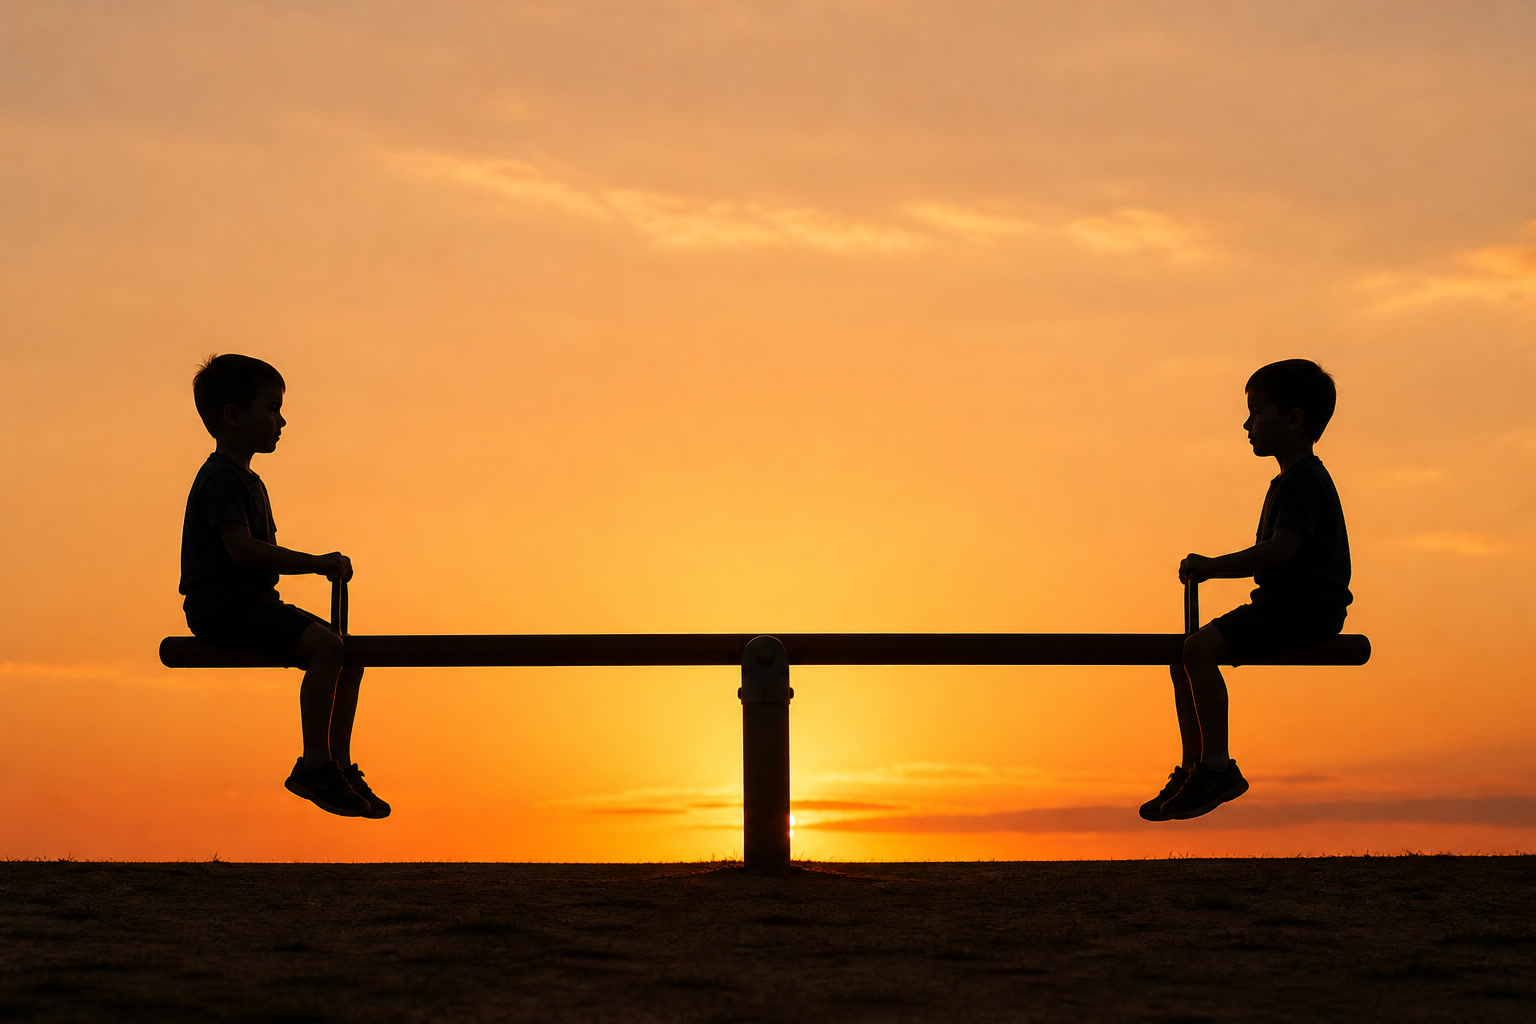
\includegraphics[width=0.58\linewidth]{images/book1/ai/g2-balance-seesaw.jpg}

{\small 操场上的完美平手：两名体型相同的骑手，坐在同样远的位置，跷跷板保持水平。}
\end{omfigure}

\begin{proposition}[跷跷板规律]\label{prop:g2:balance-equilibrium:rule}
与支点距离相等的相同重量，彼此平衡。较重的
骑手会使跷跷板倾斜——除非较重的骑手靠近
支点，或较轻的骑手向外远离。重量\emph{与}
距离都起作用。
\end{proposition}

\begin{omfigure}
\begin{tikzpicture}[scale=0.85]
  \draw[thick, fill=omExo, fill opacity=0.3]
    (2.6,0) -- (3.0,0.75) -- (2.2,0.75) -- cycle;
  \draw[very thick] (0.2,0.8) -- (5.0,0.8);
  \fill[omDef] (0.55,1.1) circle (0.26);
  \fill[omDef] (4.65,1.1) circle (0.26);
  \node[below, font=\small, align=center] at (2.6,-0.25)
    {重量相等、距离相等：\\水平};
  \draw[thick, fill=omExo, fill opacity=0.3]
    (8.9,0) -- (9.3,0.75) -- (8.5,0.75) -- cycle;
  \draw[very thick] (6.5,0.8) -- (11.3,0.8);
  \fill[omThm] (9.9,1.15) circle (0.4);
  \fill[omDef] (6.85,1.1) circle (0.26);
  \node[below, font=\small, align=center] at (8.9,-0.25)
    {重者坐近：\\再次水平};
\end{tikzpicture}

{\small 两种达到平衡的方式：重量相同、距离相同——或
较重的骑手靠近支点，对抗远处较轻的骑手。}
\end{omfigure}

\begin{remark}[一个预告]\label{rem:g2:balance-equilibrium:promise}
爸爸究竟要挪到多近？跷跷板里藏着一条
优美而精确的规律，其中还有具体的数值。它正等着
你明年在杠杆与天平一章中学习；今天的
跷跷板游戏正是它最好的预演。
\end{remark}

\section{倾倒与平衡点}

\begin{example}[倾斜过度的塔]\label{ex:g2:balance-equilibrium:tower}
搭一座积木塔，每块积木都比
下面一块伸出得稍多一些。它立着，立着\dots\ 突然倒塌。一个
倾斜的物体，当它\emph{伸出过远}，超出自身
底座时便会倒下。这就是为什么底座宽大的金字塔形积木堆很难被推倒，
而一根细高的柱子一碰就倒。宽大的底座
使积木塔稳稳当当。
\end{example}

\begin{definition}[平衡点]\label{def:g2:balance-equilibrium:point}
物体的\emph{平衡点}\index{平衡点}是指物体上的
一个特殊位置，在此托起物体，它便保持水平 --- 仿佛
全部重力都集中于此。直尺的平衡点在中间；一把
锤子的平衡点则藏在靠近较重锤头的地方。
将物体正好托在平衡点下方，它便能水平地搁在一根手指上。
\end{definition}

\begin{method}[寻找平衡点]\label{met:g2:balance-equilibrium:find}
要找出直尺、扫帚或木勺的平衡点：
\begin{enumerate}
  \item 将它横放在伸直的两根食指上，每根手指各靠近
        一端；
  \item 慢慢将两根手指相互靠拢；
  \item 两根手指会相遇 --- 物体始终保持平衡 ---
        相遇于同一点：即平衡点。
\end{enumerate}
试试扫帚：两根手指会在离中间较远的地方相遇，位于
较重的帚头一侧。平衡点总是偏向较重的一侧。
\end{method}

\begin{omfigure}
\begin{tikzpicture}[scale=0.85]
  \draw[thick, fill=omMeth, fill opacity=0.4]
    (0.3,1.5) rectangle (6.3,1.78);
  \draw[thick] (1.1,0.6) -- (1.1,1.45) (5.5,0.6) -- (5.5,1.45);
  \draw[-Stealth, omExo, thick] (1.45,0.9) -- (2.6,0.9);
  \draw[-Stealth, omExo, thick] (5.15,0.9) -- (4.0,0.9);
  \node[below, font=\small] at (3.3,0.45)
    {双指向内滑动\dots};
  \draw[thick, fill=omMeth, fill opacity=0.4]
    (7.6,1.5) rectangle (11.6,1.78);
  \draw[thick] (9.6,0.6) -- (9.6,1.45);
  \fill[omThm] (9.6,1.92) circle (2.2pt);
  \node[below, font=\small] at (9.6,0.45)
    {\dots{}两指在平衡点下方相遇};
\end{tikzpicture}

{\small 双指技巧：滑动的手指最终总会停在
平衡点的正下方。}
\end{omfigure}

\begin{example}[走钢丝者的长杆]\label{ex:g2:balance-equilibrium:acrobat}
走钢丝的人为什么要扛着那根长长下垂的杆子？它是
她的平衡帮手：当她开始向一侧倾斜时，长杆
使倾斜变得缓慢而非急促，给她留出时间
把身体重新移回绳索之上。你沿路缘走路时，用的也是同样的办法：只靠
赤手张开双臂 --- 摇晃减缓，
平衡得以保住。
\end{example}

\section{练习}

\begin{exercise}[$\star$]\label{exo:g2:balance-equilibrium:1}
桌上的台灯静止不动。写出作用在它上面的两个力，
并说明它为什么不动。
\end{exercise}

\begin{exercise}[$\star$]\label{exo:g2:balance-equilibrium:2}
拔河时，绸带在什么情况下处于平衡？是什么
打破了这种僵持？
\end{exercise}

\begin{exercise}[$\star$]\label{exo:g2:balance-equilibrium:3}
两个体重相同的双胞胎坐在跷跷板上，离支点距离相等。跷跷板会
怎样运动？其中一人向后挪，离支点更远，
此时哪一侧会下降？
\end{exercise}

\begin{exercise}[$\star$]\label{exo:g2:balance-equilibrium:4}
爸爸比莉娜重得多，可他们的跷跷板仍然水平。爸爸
应坐在哪里？请说出能让游戏顺利进行的那条规则。
\end{exercise}

\begin{exercise}[$\star$]\label{exo:g2:balance-equilibrium:5}
直尺的平衡点在哪里？锤子呢 --- 偏向
手柄一端，还是较重的锤头？怎样用一根
手指来检验？
\end{exercise}

\begin{exercise}[$\star$]\label{exo:g2:balance-equilibrium:6}
做一做\cref{met:g2:balance-equilibrium:find}中的双指技巧，
用扫帚试一试。两根手指在哪一侧相遇，
这说明了什么？
\end{exercise}

\begin{exercise}[$\star$]\label{exo:g2:balance-equilibrium:7}
哪一个更稳？为什么？是底部宽大的积木金字塔，
还是同样高、只有一块积木宽的塔？
\end{exercise}

\begin{exercise}[$\star$]\label{exo:g2:balance-equilibrium:8}
走钢丝的人为什么要拿一根长杆？沿路缘走路时，
你该如何摆动双臂？为什么这样能帮助保持平衡？
\end{exercise}

\begin{exercise}[$\star$]\label{exo:g2:balance-equilibrium:9}
右肩和右脚紧贴着一面墙站立，
墙，试着抬起左脚。你抬不起来 --- 否则
就会摔倒！请借助
\cref{ex:g2:balance-equilibrium:tower}中的塔来解释：身体要怎样
调整才能用右脚保持平衡？墙壁又限制了什么？
\end{exercise}

\begin{exercise}[$\star\star$]\label{exo:g2:balance-equilibrium:10}
建筑工地上的起重机用长长的前臂吊起重物，
--- 却不会翻倒。它较短的后臂上放着巨大的
混凝土块。请用跷跷板规则（见
\cref{prop:g2:balance-equilibrium:rule}）解释这台起重机：
两端的负载各是什么，以及为什么后臂要短？
\end{exercise}
